% Use only LaTeX2e, calling the article.cls class and 12-point type.

\documentclass[12pt]{article}

% Users of the {thebibliography} environment or BibTeX should use the
% scicite.sty package, downloadable from *Science* at
% www.sciencemag.org/about/authors/prep/TeX_help/ .
% This package should properly format in-text
% reference calls and reference-list numbers.

\usepackage{scicite}

% Use times if you have the font installed; otherwise, comment out the
% following line.

\usepackage{times}
\usepackage{graphicx}

% The preamble here sets up a lot of new/revised commands and
% environments.  It's annoying, but please do *not* try to strip these
% out into a separate .sty file (which could lead to the loss of some
% information when we convert the file to other formats).  Instead, keep
% them in the preamble of your main LaTeX source file.


% The following parameters seem to provide a reasonable page setup.

\topmargin 0.0cm
\oddsidemargin 0.2cm
\textwidth 16cm 
\textheight 21cm
\footskip 1.0cm


%The next command sets up an environment for the abstract to your paper.

\newenvironment{sciabstract}{
\begin{quote} \bf}
{\end{quote}}


% If your reference list includes text notes as well as references,
% include the following line; otherwise, comment it out.

\renewcommand\refname{References and Notes}

% The following lines set up an environment for the last note in the
% reference list, which commonly includes acknowledgments of funding,
% help, etc.  It's intended for users of BibTeX or the {thebibliography}
% environment.  Users who are hand-coding their references at the end
% using a list environment such as {enumerate} can simply add another
% item at the end, and it will be numbered automatically.

\newcounter{lastnote}
\newenvironment{scilastnote}{%
\setcounter{lastnote}{\value{enumiv}}%
\addtocounter{lastnote}{+1}%
\begin{list}%
{\arabic{lastnote}.}
{\setlength{\leftmargin}{.22in}}
{\setlength{\labelsep}{.5em}}}
{\end{list}}


% Include your paper's title here

\title{Verteilte Disparit\"atsberechnung mit WebServices und Base64 Encoding} 


% Place the author information here.  Please hand-code the contact
% information and notecalls; do *not* use \footnote commands.  Let the
% author contact information appear immediately below the author names
% as shown.  We would also prefer that you don't change the type-size
% settings shown here.

\author
{Peter Kathmann,$^{1\ast}$ Anton Antonenko,$^{1}$ Martin Hepke$^{2}$\\
\\
\normalsize{$^{1}$Systemarchitekturen f\"ur Verteilte Systeme, Technische Universit\"at Braunschweig,}\\
%\normalsize{An Unknown Address, Wherever, ST 00000, USA}\\
%\normalsize{$^{2}$Another Unknown Address, Palookaville, ST 99999, USA}\\
\\
% \normalsize{$^\ast$To whom correspondence should be addressed; E-mail:  jsmith@wherever.edu.}
}

% Include the date command, but leave its argument blank.

\date{}



%%%%%%%%%%%%%%%%% END OF PREAMBLE %%%%%%%%%%%%%%%%



\begin{document} 

% Double-space the manuscript.

\baselineskip18pt

% Make the title.

\maketitle 



% Place your abstract within the special {sciabstract} environment.

\begin{sciabstract}
In der hier vorliegenden Ausarbeitung wird die Erzeugung von Disparit\"atsbildern von zwei Stereoskopischen Bildern \"uber ein verteiltes Netzwerk betrachtet. Mittels CUDA Programmiertechnik wird die Berechnung auf mehrere Grafikprozessoren aufgeteilt. Dieses Paper betrachtet die Effizienz des Systems, wenn die Daten\"ubertragung zwischen den Rechnern mittels einer Base64-Verschl\"usselung stattfindet.
\end{sciabstract}

\newpage

\section{Einf\"uhrung}

Das hier pr\"asentierte Paper behandelt die im Seminar {\it Distributed Filesystem} aufgetragene Anpassung des bestehenden Systems zur Ermittlung von Disparit\"ats-Karten aus zwei vorliegenden Stereobildern. Das vorgegebene System operiert mittels CUDA und gsoap \"uber ein Netzwerk von Rechnern um die rechenaufw\"andige Aufgabe in kleinere Teilaufgaben zu unterteilen und damit die Rechenzeit insgesamt zu verk\"urzen.
Im Seminar wurde eine Anpassung bzw. Verbesserung des Systems von Seiten der Teilnehmer gefordert, was zentraler Bestandteil dieser Ausarbeitung ist. Unsere Gruppe {\it ``EinCooler Name''} entschied sich daf\"ur, die Daten, die vom Server an die angemeldeten Clienten weitergeleitet werden, nicht im XML-Format zu versenden sondern stattdessen die Bildwerte im das Base64 Format zu verschicken und vor ort wieder in Bildinformationen zur\"uck zu konvertieren. Als erhofftes Ergebnis war eine Laufzeitverringerung erhofft, die durch das Aussetzen einer aufwendigen XML-Konvertierung auftreten sollte.\\\\
Das Nachfolgenden Paper beschreibt dies in den folgenden Kapiteln. Im Kapitel Aufbau wird auf den Kontext der Entwicklung und der anschlie{\"ss}enden Tests eingegangen. Daraufhin folgt im Kapitel Implementierung eine Beschreibung vom programmiertechnisch Aufwand und Entscheidungen. Es folgt eine Beschreibung des Testverlaufs und der Ergebnisse im Kapitel Durchf\"uhrung. Das Paper schlie{\ss}st mit dem Kapitel Fazit und beschreibt auf Basis der Testerwerte das Ergebnis dieser Ausarbeitung und ob die urspr\"ungliche Idee zu einem Erfolg f\"uhrte.

\section{Aufbau}

Im folgenden Abschnitt findet eine Beschreibung der verwendeten Hardware und des allgemeinen Testfalls statt.\\

Entwickelt und getestet wurde das System an drei Rechnern des G40 CIP-Pools mit identischen Spezifikationen. Es waren Rechner mit einem Intel Core i7 CPU mit 8 x 4 GHz. Eine Nvidia Geforce GTX 1080 war als Grafikprozessor in Jedem eingebaut. Das Betriebssystem war ein 64bit Ubuntu 16.04 LTS mit 31,2 GiB Arbeitsspeicher.\\\\
F\"ur jeden Testdurchlauf wurde, zum Zweck der Vergleichbarkeit, das gleiche Testbild bzw. das gleiche Testbild-Paar von Stereobildern benutzt. Die Wahl fiel auf das Bild "Horse". Zu Beginn folgten diverse Testdurchl\"aufe mit dem gegebenen System um Grunddaten zu erhalten. Bei jedem Durchlauf wurden verschiedene Parameter-Kombinationen eingestellt, um ihre Wirkung auf die Laufzeit zu erfassen. Ge\"andert wurden bei jedem Durchlauf die Parameter Tau und die Skalierung. Betrachtet und notiert wurde bei den ausgegebenen Ergebnissen nur die Zeit.\\\\
Es folgten die Testdurchl\"aufe mit dem angepassten System mit der Base64 Encodierung. F\"ur jeden Durchlauf wurden die gleichen Einstellungen f\"ur die Parameter genutzt wie bei dem ersten Durchlauf, um auch hier den Einfluss der Parameter auf die Zeit zu erfassen. Die ben\"otigte Zeit des Systems wurde pro Durchlauf erfasst und mit dem des urspr\"unglichen Systems verglichen.

\section{Implementierung}
Im folgenden Kapitel wird die Implementierung der Schnittstelle n\"aher betrachtet. 
Zun\"achst wird die bestehende Schnittstelle analysiert und es wird definiert, 
welche \"Anderungen durchzuf\"uhren sind. Anschließend wird die Implementierung 
der \"Anderungen n\"aher untersucht, bevor im folgenden Kapitel die Ergebnisse betrachtet 
und ausgewertet werden.

\subsection{Ausgangslage}
Wie in der Einleitung beschrieben, sollte eine bestehende Softwarel\"osung abge\"andert werden.
In der bestehenden L\"osung wurde die verteilte Ausf\"uhrung der CUDA-Berechnungen \"uber SOAP-Requests 
eingeleitet, welche die Bilddaten als Array von Integern beinhalteten. Die prim\"aren Nachteile
der \"Ubertragung der Bilddaten als Array von Integern liegen darin, dass zum Einen ein erh\"ohter
Netwerk-Traffic anf\"allt, zum Anderen auch ein nicht unerheblicher Aufwand durch das Auswerten
der XML-Daten entsteht.\\
Der erh\"ohte Netzwerk-Traffic l\"asst sich auf die Struktur von XML-Dokumenten
zur\"uckf\"uhren, welche pro Datum ein \"offnendes und ein schließendes Tag ben\"otigen. Da es sich bei den 
Daten um ein Graustufen handelt, werden Integer \"ubertragen, die im Allgemeinen nicht mehr als drei
Stellen beinhalten. In diesem Fall bestehen die Tags jeweils aus mehr Zeichen als der zu \"ubertragende
Wert. Hierdurch entsteht ein nicht zu vern\"achl\"assigender Overhead, welcher bei einer \"Ubertragung als
Base64-Codiertes Datum minimiert wird, da die Tags nur ein mal pro Bild \"ubertragen werden m\"ussen.\\
Der Aufwand, welcher durch die Auswertung der XML-Daten entsteht, ist daher nicht unerheblich, da zum einen
die Daten als Strings vorliegen, welche in Integer konvertiert werden m\"ussen. Zum anderen jedoch bei 
SOAP-Schnittstellen im Allgemeinen auch eine Validierung der Daten vorgenommen wird. Aufgrunddessen sollte
klar sein, warum die \"Ubertragung der Bilder als Arrays einzelner Integer einen höheren Aufwand erzeugt, als die 
\"Ubertragung zweier Base64-Codierter Strings.

\subsection{Durchf\"uhrung}
In diesem Abschnitt wird die Durchf\"uhrung der im vorherigen Kapitel beschriebenen \"Anderungen erkl\"art.
Die vorzunehmenden \"Anderungen lassen sich in zwei Teilschritte unterteilen. Zum einen die Anpassung der
SOAP-Schnittstelle und zum anderen die Konvertierung der Bilddaten in Base64.\\
Um die SOAP-Schnittstelle anzupassen wurde die WSDL dahingehend geändert, dass die Bilder nun nicht mehr als 
Arrays einzelner Pixel \"ubertragen werden, sondern als einzelner String. Auf Basis der ge\"anderten WSDL wurden
unter Verwendung des Tools gsoap Client- und Serverseitig Code erzeugt, welcher die Abhandlung des SOAP-Prozesses
erm\"oglicht.\\
Um die Bilder als String zu \"ubertragen, m\"ussen diese noch in das Base64-Format konvertiert werden. Hierzu 
wurde eine einfach Konvertierungsfunktion implementiert. Diese Funktion liefert die bin\"aren Eingabedaten als
Base64-String zur\"uck. Bei der \"Ubertragung wird dieser String zusammen mit der Gr\"o{\ss}e des Originalbildes
versandt. Die Serverseite muss nun auf Basis der Originalgr\"o{\ss}e die Gr\"o{\ss}e der Daten als Base64-String 
errechnen und kann anschlie{\ss}end unter Zuhilfenahme der neu errechneten Base64-Gr\"o{\ss}e wieder ein Bild erzeugen.
Diese Bilder werden dann miteinander verglichen und die Ergebnisse werden weiterhin als Array von Integern an den 
Client zur\"uck gesandt.


\section{Auswertung}
Im folgenden Kapitel werden die Messergebnisse der vorhandenen WebService Implementierung und der modifizierten Version mit Base64-Encoding verglichen. 
Dazu wird zuerst die Testumgebung sowie die Einstellungen die wir vorgenommen haben vorgestellt auf der wir die Implementierungen ausgef\"uhrt haben. 

\subsection{Testumgebung}
Dieser Abschnitt soll die Umgebung in Einstellungen mit denen wir die Implementierungen gegeneinander getestet haben beschreiben.\\
Die Testsysteme waren 3 Computer mit folgenden Spezifikationen:

\begin{description}
\item[CPU] Intel® Core™ i7-6700K CPU @ 4.00GHz × 8 
\item[GPU] GeForce GTX 1080
\item[RAM] 31.2 GiB
\item[OS] Ubuntu 16.04 TLS
\end{description}

F\"ur alle Tests wurden die gleichen Bilder genutzt: (horse\_left\_886x818.raw, horse\_right\_886x818.raw) in 3 unterschiedlichen Aufl\"osungen
 (100\%, 70\%, 30\%).Bei 100\% und 30\% Aufl\"osung wurde die Fenstergr\"oße 15x15 und TauMax von 40 gew\"ahlt. 
 Um zu pr\"ufen wie der Einfluss der Fenstergr\"o{\ss}e und des TauMax Wertes ist wurden 3 verschiedene Kobinationen f\"ur die Aufl\"osung 70\% gew\"ahlt:\\

\begin{description}
\item[Settings A:] Tau 20 - Fenster 7x7
\item[Settings B:] Tau 40 - Fenster 7x7
\item[Settings C:] Tau 20 - Fenster 15x15
\end{description}

 

\subsection{Messergebnisse}
In diesem Abschnitt werden die Messergebnisse vorgestellt. 

\begin{figure}[ht] 
\centering 
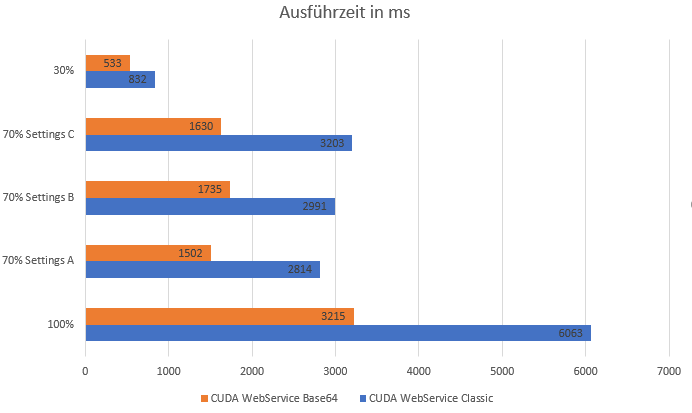
\includegraphics[scale=0.8]{Vergleich}  
\caption{Messergebnisse} 
\end{figure}

Anhand der Ergebnisse kann man sehen, dass selbst bei einer geringen Aufl\"osung des Ausgangsbildes von 30\%, 
eine Reduktion der Ausf\"uhrzeit von etwa 35\% erreicht wird, bei den h\"ohereh Aufl\"osungen sogar 42-49\%{}.
Die Base64-Implementierung kodiert und dekodiert die Rohdaten und erh\"oht deren Gr\"o\ss{}e um 33–36 \%,
dennoch ist sie fast doppelt so schnell. Das deutet darauf hin, dass der Overhead bei der Array L\"osung gr\"osser ist 
und das Parsing einzelner Bytes aufwendig.\\
M\"ochte man also nicht auf WebServices verzichten, aber trozdem eine Performance Steigerung erreichen, 
ist das \"Ubertragen eines Base64 Kodierten Strings anstatt einzelner Bytes eine Alternative die man in Betracht ziehen sollte. 

% Your references go at the end of the main text, and before the
% figures.  For this document we've used BibTeX, the .bib file
% scibib.bib, and the .bst file Science.bst.  The package scicite.sty
% was included to format the reference numbers according to *Science*
% style.


%\bibliography{scibib}

%\bibliographystyle{Science}

\end{document}
